%%%%%%%%%%%%%%%%%%%%%%%%%%%%%%%%%%%%%%%%%%%%%%%%%%%%%%%%%%%%%%%
%% OXFORD THESIS TEMPLATE

% Use this template to produce a standard thesis that meets the Oxford University requirements for DPhil submission
%
% Originally by Keith A. Gillow (gillow@maths.ox.ac.uk), 1997
% Modified by Sam Evans (sam@samuelevansresearch.org), 2007
% Modified by John McManigle (john@oxfordechoes.com), 2015
% Modified by Ulrik Lyngs (ulrik.lyngs@cs.ox.ac.uk), 2018, for use with R Markdown
%
% Ulrik Lyngs, 25 Nov 2018: Following John McManigle, broad permissions are granted to use, modify, and distribute this software
% as specified in the MIT License included in this distribution's LICENSE file.
%
% John tried to comment this file extensively, so read through it to see how to use the various options.  Remember
% that in LaTeX, any line starting with a % is NOT executed.  Several places below, you have a choice of which line to use
% out of multiple options (eg draft vs final, for PDF vs for binding, etc.)  When you pick one, add a % to the beginning of
% the lines you don't want.


%%%%% CHOOSE PAGE LAYOUT
% The most common choices should be below.  You can also do other things, like replacing "a4paper" with "letterpaper", etc.

% This one will format for two-sided binding (ie left and right pages have mirror margins; blank pages inserted where needed):
%\documentclass[a4paper,twoside]{templates/ociamthesis}
% This one will format for one-sided binding (ie left margin > right margin; no extra blank pages):
%\documentclass[a4paper]{ociamthesis}
% This one will format for PDF output (ie equal margins, no extra blank pages):
%\documentclass[a4paper,nobind]{templates/ociamthesis}
%UL 2 Dec 2018: pass this in from YAML
\documentclass[a4paper, nobind]{templates/ociamthesis}


% UL 30 Nov 2018 pandoc puts lists in 'tightlist' command when no space between bullet points in Rmd file
\providecommand{\tightlist}{%
  \setlength{\itemsep}{0pt}\setlength{\parskip}{0pt}}
 
% UL 1 Dec 2018, fix to include code in shaded environments

%UL 2 Dec 2018 reduce whitespace around verbatim environments
\usepackage{etoolbox}
\makeatletter
\preto{\@verbatim}{\topsep=0pt \partopsep=0pt }
\makeatother

%UL 26 Mar 2019, enable strikethrough
\usepackage[normalem]{ulem}

%UL 15 Oct 2019, enable link highlighting to be turned off from YAML
\usepackage[colorlinks=false,pdfpagelabels,hidelinks=true]{hyperref}

%%%%% SELECT YOUR DRAFT OPTIONS
% Three options going on here; use in any combination.  But remember to turn the first two off before
% generating a PDF to send to the printer!

% This adds a "DRAFT" footer to every normal page.  (The first page of each chapter is not a "normal" page.)

% This highlights (in blue) corrections marked with (for words) \mccorrect{blah} or (for whole
% paragraphs) \begin{mccorrection} . . . \end{mccorrection}.  This can be useful for sending a PDF of
% your corrected thesis to your examiners for review.  Turn it off, and the blue disappears.
\correctionstrue

%%%%% BIBLIOGRAPHY SETUP
% Note that your bibliography will require some tweaking depending on your department, preferred format, etc.
% The options included below are just very basic "sciencey" and "humanitiesey" options to get started.
% If you've not used LaTeX before, I recommend reading a little about biblatex/biber and getting started with it.
% If you're already a LaTeX pro and are used to natbib or something, modify as necessary.
% Either way, you'll have to choose and configure an appropriate bibliography format...

% The science-type option: numerical in-text citation with references in order of appearance.
% \usepackage[style=numeric-comp, sorting=none, backend=biber, doi=false, isbn=false]{biblatex}
% \newcommand*{\bibtitle}{References}

% The humanities-type option: author-year in-text citation with an alphabetical works cited.
% \usepackage[style=authoryear, sorting=nyt, backend=biber, maxcitenames=2, useprefix, doi=false, isbn=false]{biblatex}
% \newcommand*{\bibtitle}{Works Cited}

%UL 3 Dec 2018: set this from YAML in index.Rmd
\usepackage[style=authoryear, sorting=nyt, backend=biber, maxcitenames=2, useprefix, doi=true, isbn=false, uniquename=false]{biblatex}
\newcommand*{\bibtitle}{Works Cited}

% This makes the bibliography left-aligned (not 'justified') and slightly smaller font.
\renewcommand*{\bibfont}{\raggedright\small}

% Change this to the name of your .bib file (usually exported from a citation manager like Zotero or EndNote).
\addbibresource{references.bib}


% Uncomment this if you want equation numbers per section (2.3.12), instead of per chapter (2.18):
%\numberwithin{equation}{subsection}


%%%%% THESIS / TITLE PAGE INFORMATION
% Everybody needs to complete the following:
\title{Analyzing the Feature Importance of Different Variables on the Price of Ikea Products}
\author{Philip Krück, Johannes Pein}
\college{}

% Master's candidates who require the alternate title page (with candidate number and word count)
% must also un-comment and complete the following three lines:
%\masterssubmissiontrue
%\candidateno{933516}
%\wordcount{28,815}

% Uncomment the following line if your degree also includes exams (eg most masters):
%\renewcommand{\submittedtext}{Submitted in partial completion of the}
% Your full degree name.  (But remember that DPhils aren't "in" anything.  They're just DPhils.)
\degree{B.Sc. Business Informatics (18A-BI)}
% Term and year of submission, or date if your board requires (eg most masters)
\degreedate{04.12.2020}


%%%%% YOUR OWN PERSONAL MACROS
% This is a good place to dump your own LaTeX macros as they come up.
\modulename{Digital Toolbox: Data Business}
\lecturer{Lecturer: Ulf Köther}
\groupnumber{Group Number: 7}
\matriculationnumbers{Matriculation Numbers: 3938 (P.Krück), 4001 (J.Pein)}


% To make text superscripts shortcuts
	\renewcommand{\th}{\textsuperscript{th}} % ex: I won 4\th place
	\newcommand{\nd}{\textsuperscript{nd}}
	\renewcommand{\st}{\textsuperscript{st}}
	\newcommand{\rd}{\textsuperscript{rd}}

%%%%% THE ACTUAL DOCUMENT STARTS HERE
\begin{document}

%%%%% CHOOSE YOUR LINE SPACING HERE
% This is the official option.  Use it for your submission copy and library copy:
\setlength{\textbaselineskip}{22pt plus2pt}
% This is closer spacing (about 1.5-spaced) that you might prefer for your personal copies:
%\setlength{\textbaselineskip}{18pt plus2pt minus1pt}

% You can set the spacing here for the roman-numbered pages (acknowledgements, table of contents, etc.)
\setlength{\frontmatterbaselineskip}{17pt plus1pt minus1pt}


% UL: You can set the general paragraph spacing here - I've set it to 2pt (was 0) so
% it's less claustrophobic
\setlength{\parskip}{2pt plus 1pt}


% Leave this line alone; it gets things started for the real document.
\setlength{\baselineskip}{\textbaselineskip}


%%%%% CHOOSE YOUR SECTION NUMBERING DEPTH HERE
% You have two choices.  First, how far down are sections numbered?  (Below that, they're named but
% don't get numbers.)  Second, what level of section appears in the table of contents?  These don't have
% to match: you can have numbered sections that don't show up in the ToC, or unnumbered sections that
% do.  Throughout, 0 = chapter; 1 = section; 2 = subsection; 3 = subsubsection, 4 = paragraph...

% The level that gets a number:
\setcounter{secnumdepth}{2}
% The level that shows up in the ToC:
\setcounter{tocdepth}{2}


% JEM: Pages are roman numbered from here, though page numbers are invisible until ToC.  This is in
% keeping with most typesetting conventions.
\begin{romanpages}

% Title page is created here
\maketitle

%%%%% MINI TABLES
% This lays the groundwork for per-chapter, mini tables of contents.  Comment the following line
% (and remove \minitoc from the chapter files) if you don't want this.  Un-comment either of the
% next two lines if you want a per-chapter list of figures or tables.
  \dominitoc % include a mini table of contents

% This aligns the bottom of the text of each page.  It generally makes things look better.
\flushbottom

% This is where the whole-document ToC appears:
\tableofcontents

%%%%% LIST OF ABBREVIATIONS
% This example includes a list of abbreviations.  Look at text/abbreviations.tex to see how that file is
% formatted.  The template can handle any kind of list though, so this might be a good place for a
% glossary, etc.
% First parameter can be changed eg to "Glossary" or something.
% Second parameter is the max length of bold terms.
\begin{mclistof}{List of Abbreviations}{3.2cm}

\item[R] Statistical Programming Language
\item[MSE] Mean Squared Error
\item[IQR] Interquartile Range

\end{mclistof} 


% The Roman pages, like the Roman Empire, must come to its inevitable close.
\end{romanpages}

%%%%% CHAPTERS
% Add or remove any chapters you'd like here, by file name (excluding '.tex'):
\flushbottom

% all your chapters and appendices will appear here
\hypertarget{intro}{%
\chapter{Introduction}\label{intro}}

\begin{figure}
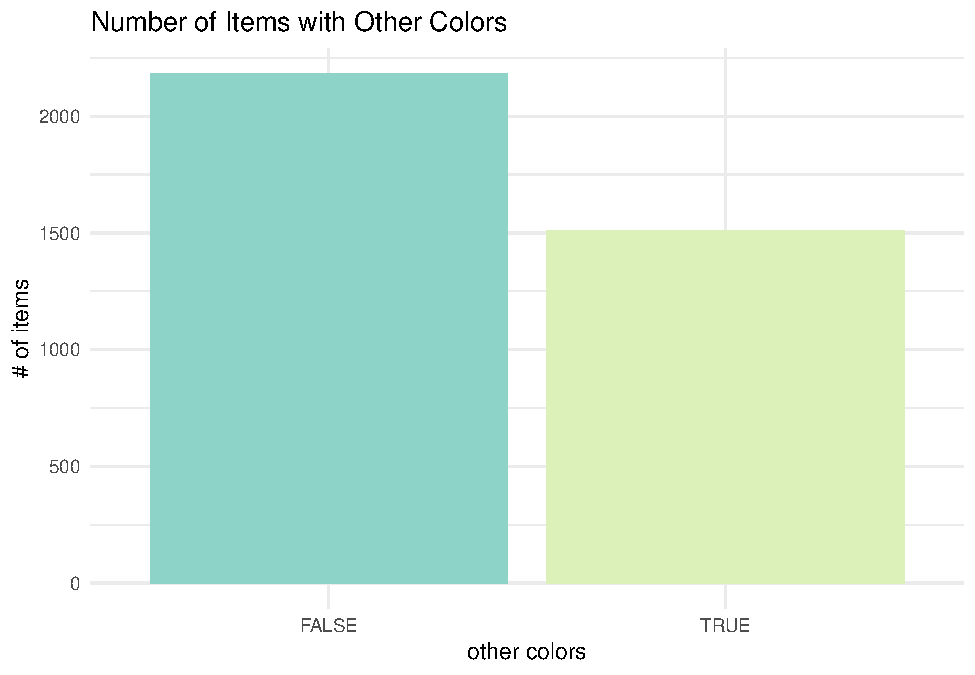
\includegraphics[width=1\linewidth]{_main_files/figure-latex/unnamed-chunk-3-1} \caption{Sample plot}\label{fig:unnamed-chunk-3}
\end{figure}

\hypertarget{theoretical-background-research-question}{%
\chapter{Theoretical Background \& Research Question}\label{theoretical-background-research-question}}

\hypertarget{theoretical_background}{%
\section{Theoretical Background}\label{theoretical_background}}

\hypertarget{data-set}{%
\subsection{Data Set}\label{data-set}}

The data set was obtained by a kaggle.com user (Reem Abdulrahman) by the means of webscraping techniques from the Saudi Arabian Ikea website in the furniture category on the 20th of April 2020. Noteworthy features include the name, category, price in Saudi Riyals, the designer and dimensions (width, height and depth). The data set has 13 variables and 2962 observations.

\hypertarget{rf-basics}{%
\subsection{RF Basics}\label{rf-basics}}

In order to analyze the feature importance in relation to the price variable, a random forest regression model was chosen. A random forest consists of many decision trees, which make a prediction based on a majority decision process. In standard decision trees, each nodes is split to achieve the best performing model. In random forests however, the nodes are randomly split. Compared to linear regression models, the random forests model not only takes into account the mean and covariance structure of response, but also deeper deeper aspects of data\footnote{Grömping, ``Variable Importance Assessment in Regression: Linear Regression versus Random Forest.''} leading to a more advanced and robust model.

\hypertarget{feature-importance}{%
\subsection{Feature Importance}\label{feature-importance}}

\begin{itemize}
\tightlist
\item
  feature and predictor variable can be used interchangibly
\end{itemize}

\hypertarget{research_question}{%
\section{Research Question}\label{research_question}}

This paper explores the influence for different variables on the price in the given data set. The motivating forces for this research question are the possible implications for price determination of new items.

\hypertarget{methods}{%
\chapter{Methods}\label{methods}}

\hypertarget{datacleaning}{%
\section{Data Cleaning and Transformatoin}\label{datacleaning}}

To examine our data set properly, we first had to restructure and reformat it. This initial data cleaning step included type conversions, value mutation, addition of new calculated fields and the dropping of irrelevant columns.
Concretely, we converted name, category and designer to categorical variables. In the designer column, we converted blank strings and values prefixed by ``IKEA of Sweden'' to missing values (\texttt{NA}). Furthermore, we converted both the price and old price to double values and changed the currency from Saudi Arabian Riyals to Euros based on the exchange rate from the time the data set was obtained by the author @ref(\#theoretical\_background). To better facilitate the comparison of the different sizes of furniture items, we calcuted the size in cubic meters based on the depth, width and height values.
Finally, we selected only columns that could have a potential impact in our analysis (see Table \ref{tab:initial-ikea} and \ref{tab:tidy-ikea}).

tidy category -\textgreater{} duplicate filtering
- there were some observations with the same item id. All other value were the same in these instances except for the category.
- The authors considered multiple approaches to handle these data duplications
- Option one -\textgreater{} mutate duplicates into one combination of categories (e.g.~a and b to a, b), then the newly created categories would have a low count of observations while the single categories would have a decreased count. We would then have an increased count in categories. Because the count of the individual categories is low, no definite conclusion can be drawn for the interaction on the price
- Option two -\textgreater{} create multiple variables for each observed category for the same item id. The authors wanted to analyze the feature importance of category variable as such and not the multiple occurrences of the category variable
- The authors chose option of selecting the observations where the category count occurred most frequent.

TODO: Format these tables

\begin{table}

\caption{\label{tab:initial-ikea}Initial Data Set formatting.}
\centering
\begin{tabular}[t]{r|r|l|l|r|l|l|l|l|l|l|r|r|r}
\hline
X1 & item\_id & name & category & price & old\_price & sellable\_online & link & other\_colors & short\_description & designer & depth & height & width\\
\hline
0 & 90420332 & FREKVENS & Bar furniture & 2650 & No old price & TRUE & https://www.ikea.com/sa/en/p/frekvens-bar-table-in-outdoor-black-90420332/ & No & Bar table, in/outdoor,          51x51 cm & Nicholai Wiig Hansen & NA & 99 & 51\\
\hline
1 & 368814 & NORDVIKEN & Bar furniture & 9950 & No old price & FALSE & https://www.ikea.com/sa/en/p/nordviken-bar-table-black-00368814/ & No & Bar table,          140x80 cm & Francis Cayouette & NA & 105 & 80\\
\hline
2 & 9333523 & NORDVIKEN / NORDVIKEN & Bar furniture & 20950 & No old price & FALSE & https://www.ikea.com/sa/en/p/nordviken-nordviken-bar-table-and-4-bar-stools-black-black-s09333523/ & No & Bar table and 4 bar stools & Francis Cayouette & NA & NA & NA\\
\hline
3 & 80155205 & STIG & Bar furniture & 690 & No old price & TRUE & https://www.ikea.com/sa/en/p/stig-bar-stool-with-backrest-black-silver-colour-80155205/ & Yes & Bar stool with backrest,          74 cm & Henrik Preutz & 50 & 100 & 60\\
\hline
4 & 30180504 & NORBERG & Bar furniture & 2250 & No old price & TRUE & https://www.ikea.com/sa/en/p/norberg-wall-mounted-drop-leaf-table-white-30180504/ & No & Wall-mounted drop-leaf table,          74x60 cm & Marcus Arvonen & 60 & 43 & 74\\
\hline
5 & 10122647 & INGOLF & Bar furniture & 3450 & No old price & TRUE & https://www.ikea.com/sa/en/p/ingolf-bar-stool-with-backrest-white-10122647/ & No & Bar stool with backrest,          63 cm & Carina Bengs & 45 & 91 & 40\\
\hline
\end{tabular}
\end{table}

\begin{table}

\caption{\label{tab:tidy-ikea}Data Set after cleaning process.}
\centering
\begin{tabular}[t]{l|l|r|r|l|l|l|r}
\hline
name & category & price\_eur & old\_price\_eur & sellable\_online & other\_colors & designer & size\_m3\\
\hline
FREKVENS & Bar furniture & 65.02 & NA & TRUE & FALSE & Nicholai Wiig Hansen & NA\\
\hline
NORDVIKEN & Bar furniture & 244.14 & NA & FALSE & FALSE & Francis Cayouette & NA\\
\hline
NORDVIKEN / NORDVIKEN & Bar furniture & 514.05 & NA & FALSE & FALSE & Francis Cayouette & NA\\
\hline
STIG & Bar furniture & 16.93 & NA & TRUE & TRUE & Henrik Preutz & 0.30\\
\hline
NORBERG & Bar furniture & 55.21 & NA & TRUE & FALSE & Marcus Arvonen & 0.19\\
\hline
INGOLF & Bar furniture & 84.65 & NA & TRUE & FALSE & Carina Bengs & 0.16\\
\hline
\end{tabular}
\end{table}

\hypertarget{tbd}{%
\section{8 Step EDA (nice heading)}\label{tbd}}

\footnote{Zuur, ``A protocol for data exploration to avoid common statistical problems,'' 33--35.}.
- Our EDA analysis is based on the protocol for data exploration proposed by ZUUR paper
- This 8 step analysis is especially useful for regression models

\hypertarget{step-1-outliers-in-price-and-independent-variables}{%
\subsection{Step 1: Outliers in Price and Independent Variables}\label{step-1-outliers-in-price-and-independent-variables}}

\begin{itemize}
\tightlist
\item
  Assumption: outliers are not by chance or random (no observer error)
\item
  Assumption seems to hold up when looking at individual outlier observations. These are congruent in themselves. Assume: web scraping technique is highly unlikely to have measurement error ocurrence
\item
  Use outliers in model
\end{itemize}

\hypertarget{step-2-homogeneity-of-price}{%
\subsection{Step 2: Homogeneity of Price}\label{step-2-homogeneity-of-price}}

\begin{itemize}
\tightlist
\item
  To test the assumption of homogeneity of variance for price (homoscedasticity) by the means of conditional boxplotting
\item
  As can be seen, price is homogoneous for all category variable except for beds where the variance differes widely (see plot xxx)
\item
  price is heterogenous for all individual names by category (see plot xxx)
\item
  Looking at both categories simultaneously -\textgreater{} homogenous
\item
  Im Rahmen der Arbeit nicht möglich alle kategorischen Variablen Kombinationen anzuschauen. 5 kategorische Variablen -\textgreater{} 2\^{}5 = 32 Möglichkeiten
\end{itemize}

\hypertarget{step-3-missing-value-trouble}{%
\subsection{Step 3: Missing Value Trouble}\label{step-3-missing-value-trouble}}

\begin{itemize}
\tightlist
\item
  not normal verteilt
\item
  ikea ist im Niedrigpreissegment angesiedelt
\item
  see figure \ldots{}.
\item
  exponential decay in price, old price and size (e\^{}-x)
\end{itemize}

\hypertarget{zeros}{%
\subsection{Step 4: Zeros}\label{zeros}}

\begin{itemize}
\tightlist
\item
  many missing values from old price -\textgreater{} assume those were not on sale
\item
  size\_m3 missing values because of calculation formula
\item
  designer -\textgreater{} removed values containing digits (were clearly falsely scraped)
\end{itemize}

\hypertarget{collinearity}{%
\subsection{Step 5: Collinearity between Independent Variables}\label{collinearity}}

\begin{itemize}
\tightlist
\item
  high collinearity between old price and price
\item
  relatively high collinearity between price and size
\item
  as can be seen in table
\end{itemize}

\hypertarget{relationship}{%
\subsection{Step 6: Relationship between Independent Variables and Price}\label{relationship}}

\begin{itemize}
\tightlist
\item
  from eda\_covariance.Rc (in Anhang + verweisen)
\item
  strong relationship b/w price + old price \& b/w price + size (see )
\item
  other relationships aren't strong
\end{itemize}

\hypertarget{step-7-interactions}{%
\subsection{Step 7: Interactions}\label{step-7-interactions}}

\begin{itemize}
\item
  Coplotting designer and name works, while the two combination would not plot
\item
  The linear model predicted infinite values and thus coplot the values properly for the other two options
\item
  However, dropping all NA values and thus reducing the total data size to 354 observations would case for the combination coplot name and category while name + designer combination would not work
\item
  The authors hypothesized that infinite values were caused by a division of zeros of the linear model since there occured 0 values in size
\item
  This however proved to be wrong after applying respective filters
\item
  The following interaction could be analyzed
\item
  \begin{itemize}
  \tightlist
  \item
    There is probably no significant interaction between size, price, name \& designer as can be seen in coplot -\textgreater{} lines are nearly parallel
  \end{itemize}
\item
  Based on the coplot of category and name with the 354 observations, inparallelity could be observed and thus could conclude a interaction. However, this could also be due to the small sample size
\item
\end{itemize}

(footnote): the authors would highly appreciate any solutions on this matter\footnote{This is a footnote.}

\hypertarget{step-8-independence-of-price}{%
\subsection{Step 8: Independence of Price}\label{step-8-independence-of-price}}

\begin{itemize}
\tightlist
\item
  Durch das tidying in (cross reference) duplicate removal -\textgreater{} Zuur paper Step 8 1. citation: meaning that information from any one observation should not provide information on another after the effects of other variables have been accounted for. This concept is best explained with examples.
\end{itemize}

\hypertarget{rf}{%
\section{Random Forest Regression Model}\label{rf}}

This analysis was conducted using the R randomForest package, which is based on the original Breiman and Cutler's Fortran code for random forest regression. To learn more about how random forests work or the randomForest package, see Liaw and Wiener\footnote{``Classification and Regression by randomForest.''} or \#chapter2 \#TODO. To reproduce the analysis conducted in this paper, the prepatory steps are described now. The following steps are based on an already cleaned ikea data frame which is described in \ref{datacleaning}. This data frame is then transformed further to be used with the randomForest package.
First, the variable \texttt{old\_price\_eur} is removed from the data frame, due to a very high correlation and relationship to the price variable analyzed in \ref{collinearity} and \ref{relationship} Then, the designers and names, which are not part of the 50 \texttt{designers} and 49 \texttt{names} with the highest number of occurences, are grouped in the \texttt{other} value. This is because the \texttt{randomForest} method does not allow categorical variables with more than 53 predictors. The last step is dealing with the missing values in the data. As described in \ref{zeros}, there are missing values in the \texttt{size\_m3} and \texttt{designer} variables. To use the \texttt{randomForest} method of the randomForest package on the data, those missing values are dealt with using three different approaches. In the first approach the rows with missing values are deleted, reducing the total number of rows by aproximately 50\%. In the second approach the missing values are dummy coded with a value of -1000. The third approach uses the \texttt{na.roughfix\ =\ na.omit} argument, which is the built in way of the randomForest package to deal with missing values.
After preparing the data, the \texttt{randomForest} method of the randomForest package is applied to the data with number of trees set to 2000 and importance set to \texttt{TRUE}.

\texttt{randomForest(price\_eur\ \textasciitilde{}\ .,\ rf\_ikea,\ ntree=2000,\ keep.forest=FALSE,\ importance=TRUE)}

Then the \texttt{importance} method of the randomForest package is used to save the feature importances, which are computed by permuting feature importance, which is described in \#chapter2 \#TODO. The three different approaches of dealing with the missing values in the data set lead to different results, so the authors chose to calculate the mean result of the three approaches. The result of this analysis is presented in the following chapter.

\begin{itemize}
\tightlist
\item
  TODO: is normal distribution relevant for random forest (step 3) -\textgreater{} see article or cite something
\end{itemize}

\hypertarget{results}{%
\chapter{Results}\label{results}}

\hfill\textcolor{gray}{by J. Pein}

\hypertarget{todo-set-n_trees-to-2000-before-handing-in}{%
\section{TODO: set n\_trees to 2000 before handing in}\label{todo-set-n_trees-to-2000-before-handing-in}}

In this chapter, the results of the analysis of the feature importance of different predictor variables (features) on the response variable price of Ikea products are presented.

As described in \ref{rf}, the feature importance was calculated using permuting feature importance of the randomForest R package. In this analysis, feature importance is derived from the percentage increase of the mean squared error (MSE) of the overall random forest regression model with the response variable \texttt{price\_eur}. When the percentage increase of the MSE is higher, the feature is more important, accordingly, when the percentage increase of the MSE is lower, the feature is less important.

\begin{figure}
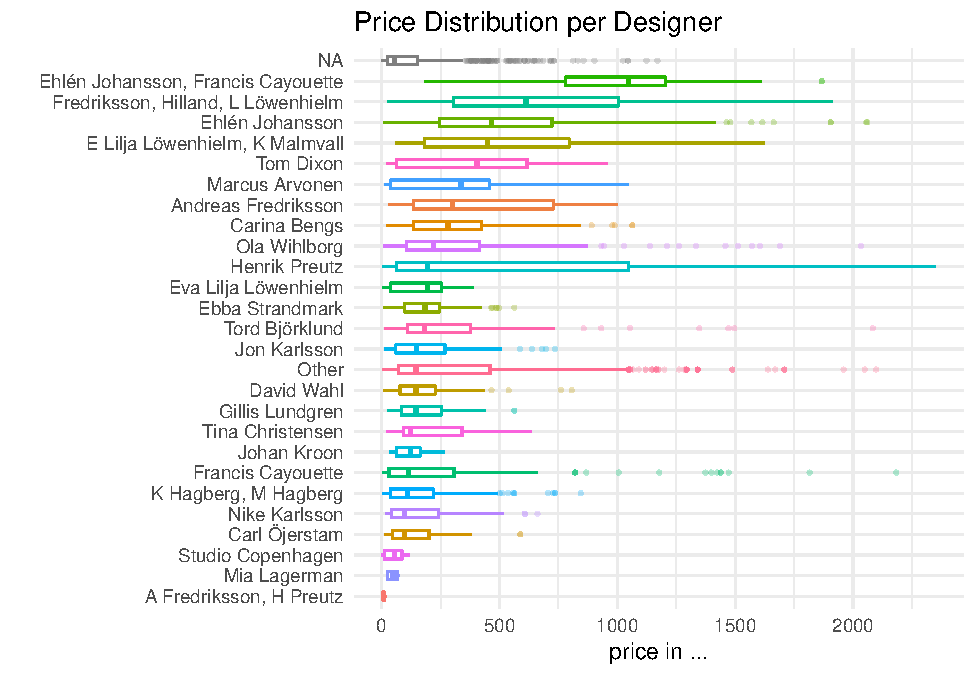
\includegraphics[width=0.9\linewidth]{_main_files/figure-latex/unnamed-chunk-5-1} \caption{A nice image.}\label{fig:unnamed-chunk-5}
\end{figure}

Thus, as can be seen in the figure above, the most important feature is \texttt{size\_m3} with an increase of the MSE of 182\%. The second, third and fourth most important features are \texttt{designer} with an increase of 120\%, \texttt{name} with an increase of 114\% and \texttt{category} with an increase of 105\%. The fifth most important feature is \texttt{other\_colors} with an increase of the MSE of 78\% and the least important feature is \texttt{sellable\_online} with a 9\% increase.

These results are further discussed in the following section.

\hypertarget{discussion}{%
\chapter{Discussion}\label{discussion}}

\hypertarget{size_m3}{%
\section{size\_m3}\label{size_m3}}

\begin{itemize}
\tightlist
\item
  material cost
\item
  big items more expensive than small ones
\item
  high correlation to price
\end{itemize}

\hypertarget{designer}{%
\section{designer}\label{designer}}

\begin{itemize}
\item
  designers with high number of products produce products in wide price range : plot reference -\textgreater{} appendix
\item
  many different combinations of designer (49-53)
\item
  many designer-combinations with low number of products:

  \begin{itemize}
  \tightlist
  \item
    n combinations with occurrences\textless{}5
  \end{itemize}
\end{itemize}

-\textgreater{} overfitting: cite scholarly article
-\textgreater{} low generalization : model might perfom bad on other data

\hypertarget{name}{%
\section{name}\label{name}}

\begin{itemize}
\tightlist
\item
  overfitting
\end{itemize}

\hypertarget{category}{%
\section{category}\label{category}}

\begin{itemize}
\tightlist
\item
  beds are more expensive than chairs : some categories are more expensive than others (show plot)
\item
  but, price range varies heavily in category (show plot)
\end{itemize}

\hypertarget{other_colors}{%
\section{other\_colors}\label{other_colors}}

\begin{itemize}
\tightlist
\item
  products of every price range have both options : low importance
\item
  mean price is higher if other\_colors is true (show plot covariance price+other\_colors)
\item
  interquartile-range is smaller if other\_colors is false
\end{itemize}

\hypertarget{sellable_online}{%
\section{sellable\_online}\label{sellable_online}}

sellable true: price range too high
sellable ntrue: very rare

\hypertarget{conclusion-ausblick}{%
\section{Conclusion \& Ausblick}\label{conclusion-ausblick}}

general results might contain bias or variance errors, further investigating

\begin{itemize}
\tightlist
\item
  Further research:

  \begin{itemize}
  \tightlist
  \item
    analyze designer overfitting, recommend using overfitting techniques (e.g. \ldots{})
  \item
    analyze same research question with other techniques (lm, name more) and compare
  \item
    data scraping from other country-pages
  \end{itemize}
\end{itemize}

\hypertarget{individual-statements}{%
\chapter{Individual Statements}\label{individual-statements}}

\hypertarget{philip-kruxfcck}{%
\section{Philip Krück}\label{philip-kruxfcck}}

\hypertarget{johannes-pein}{%
\section{Johannes Pein}\label{johannes-pein}}

\startappendices

\hypertarget{appendix}{%
\chapter{Appendix}\label{appendix}}

\hypertarget{plot-abc}{%
\section{Plot abc}\label{plot-abc}}

\hypertarget{plot-xyz}{%
\section{Plot xyz}\label{plot-xyz}}

\hypertarget{bibliography}{%
\chapter{Bibliography}\label{bibliography}}

\hypertarget{refs}{}
\leavevmode\hypertarget{ref-Groemping2009}{}%
Grömping, Ulrike. ``Variable Importance Assessment in Regression: Linear Regression versus Random Forest.'' \emph{The American Statistician}, nos. Vol. 63, No. 4 (2009): 308--19. \url{https://prof.beuth-hochschule.de/fileadmin/prof/groemp/downloads/tast_2E2009_2E08199.pdf}.

\leavevmode\hypertarget{ref-Liaw2002}{}%
Liaw, Andy, and Matthew Wiener. ``Classification and Regression by randomForest.'' \emph{R News}, nos. Vol. 2/3, December 2002 (2001). \url{https://www.researchgate.net/publication/228451484_Classification_and_Regression_by_RandomForest}.

\leavevmode\hypertarget{ref-Zuur2010}{}%
Zuur, E.N. Ieno lain. ``A protocol for data exploration to avoid common statistical problems.'' \emph{British Ecological Society}, 2010. doi:\href{https://doi.org/10.1145/1738826.1738829}{10.1145/1738826.1738829}.


%%%%% REFERENCES

% JEM: Quote for the top of references (just like a chapter quote if you're using them).  Comment to skip.
% \begin{savequote}[8cm]
% The first kind of intellectual and artistic personality belongs to the hedgehogs, the second to the foxes \dots
%   \qauthor{--- Sir Isaiah Berlin \cite{berlin_hedgehog_2013}}
% \end{savequote}

\setlength{\baselineskip}{0pt} % JEM: Single-space References

{\renewcommand*\MakeUppercase[1]{#1}%
\printbibliography[heading=bibintoc,title={\bibtitle}]}

\end{document}
